\documentclass[a4paper,13pt]{article}

% --- Tiếng Việt + mã UTF-8 ---
\usepackage[utf8]{inputenc}
\usepackage[T5]{fontenc}
\usepackage[vietnamese]{babel}

% --- Bố cục trang ---
\usepackage{geometry}
\geometry{top=2.5cm, bottom=2.5cm, left=3cm, right=2cm}

% --- Toán ---
\usepackage{amsmath}

% --- Ảnh (logo bìa + biểu đồ) ---
\usepackage{graphicx}
\graphicspath{{../experiments/figures/}}

% --- Liên kết ---
\usepackage{hyperref}

\begin{document}

% ================= TRANG BÌA =================
\begin{center}
\large ỦY BAN NHÂN DÂN THÀNH PHỐ HỒ CHÍ MINH \\[0.2cm]

\includegraphics[width=3.5cm]{SGU-LOGO.png} \\[0.4cm]
\large TRƯỜNG ĐẠI HỌC SÀI GÒN \\
\large KHOA TOÁN -- ỨNG DỤNG \\[0.3cm]
\rule{12cm}{1.5pt} \\[0.8cm]

\Large \textbf{BÁO CÁO BÀI THỰC HÀNH} \\[0.4cm]
\large Môn: Học sâu (Deep Learning) \\
\Large \textbf{Lab02: Dự báo giá nhà (House Prices)} \\[1.2cm]

\begin{tabular}{lll}
STT & Họ và tên & MSSV \\
1 & Đinh Quang Minh & 3123580024 \\
2 & Dương Tấn Cường & 3123580004 \\
3 & Lê Thành Duy & 3123580007 \\
\end{tabular}\\[0.5cm]

\begin{tabular}{ll}
Lớp: & DDU1231 \\
Ngành: & Khoa học dữ liệu \\
Giảng viên hướng dẫn: & TS. Đỗ Như Tài \\
Học kỳ: & Học kỳ I, năm học 2026 \\
\end{tabular}\\[1.5cm]

TP. Hồ Chí Minh, tháng 9 năm 2026 \\
\end{center}

\newpage
\section*{Bảng phân công nhiệm vụ}

{\small
\begin{center}
\begin{tabular}{|c|l|p{7.5cm}|c|}
\hline
\textbf{STT} & \textbf{Họ và tên} & \textbf{Nội dung thực hiện} & \textbf{Đóng góp} \\
\hline
1 & Đinh Quang Minh & EDA, pipeline xử lý dữ liệu, mô hình tuyến tính (M0--M3), tổng hợp notebook & 40\% \\
\hline
2 & Dương Tấn Cường & Mạng nơ-ron MLP, embeddings (M4--M6), fine-tune & 30\% \\
\hline
3 & Lê Thành Duy & Ensemble, nộp Kaggle, vòng lặp cải tiến, viết báo cáo & 30\% \\
\hline
\end{tabular}
\end{center}
}

\newpage
\tableofcontents
\newpage

\section{Giới thiệu bài toán}

\subsection{Mục tiêu}
Cuộc thi Kaggle \textit{House Prices -- Advanced Regression Techniques} yêu cầu dự báo giá bán
(\texttt{SalePrice}, USD) của 1459 căn nhà ở Ames, Iowa (tập test không nhãn), học từ 1460 căn
có nhãn (tập train). Đây là bài toán \textbf{hồi quy có giám sát} dựa trên bộ dữ liệu nhà đất
Ames do De Cock (2011) giới thiệu, gồm 79 biến giải thích: 23 nominal, 23 ordinal, 14 discrete
và 20 continuous, mô tả chất lượng và số lượng của căn nhà.

\subsection{Metric đánh giá: RMSLE}
Kaggle chấm bằng \textbf{RMSLE} (sai số log quân phương):
\[
\text{RMSLE} = \sqrt{\frac{1}{n}\sum_{i=1}^{n}\bigl(\log(1+\hat{y}_i)-\log(1+y_i)\bigr)^2}.
\]
RMSLE phạt sai số \textit{tương đối}: đoán lệch 10 nghìn USD trên nhà rẻ bị phạt nặng hơn cùng
mức lệch trên nhà đắt. Hệ quả thiết kế xuyên suốt bài làm: mọi huấn luyện, đánh giá và trộn mô
hình đều thực hiện trên thang $\log(1+y)$.

\subsection{Ràng buộc và tiêu chí thành công}
\begin{itemize}
  \item Toàn bộ mô hình cài đặt bằng \textbf{PyTorch} (sklearn chỉ hỗ trợ chia fold và tiền xử lý).
  \item Quy trình theo 6 bước \textbf{CRISP-DM}, mỗi mô hình fine-tune 2 vòng
        (screening nhanh rồi refine bằng 5-fold CV), mọi thí nghiệm ghi vào nhật ký.
  \item Thành công nội bộ: CV-RMSLE giảm dần qua các thí nghiệm; minh chứng triển khai:
        điểm public leaderboard khi nộp Kaggle.
\end{itemize}

\newpage
\section{Khám phá dữ liệu (EDA)}

\subsection{Phân phối giá và ô trống}
Giá bán lệch phải mạnh (skew 1.883, trung bình 181k $>$ trung vị 163k); sau
\texttt{log1p} skew chỉ còn 0.121, gần chuẩn — xác nhận quyết định làm việc trên thang log.
Trong 81 cột có 19 cột thiếu, nhưng thiếu đều có ý nghĩa: PoolQC (99.5\%),
MiscFeature (96\%), Alley (94\%), Fence (81\%) thiếu nghĩa là \textit{không có} hạng mục đó,
nên điền \texttt{'Missing'} thay vì xóa.

\begin{center}
\includegraphics[width=0.95\textwidth]{eda_gia.png} \\
\includegraphics[width=0.95\textwidth]{eda_missing_corr.png}
\end{center}

\subsection{Tương quan, khu vực và ngoại lệ}
Các biến đắt giá nhất: OverallQual (0.817), GrLivArea (0.701), GarageCars (0.681) — đúng
như paper nhấn mạnh. Heatmap cho thấy cụm Garage, cụm diện tích và OverallQual dính chùm
với nhau: đa cộng tuyến rõ, báo trước cần regularization. Hiệu ứng vị trí rất mạnh:
trung vị khu NridgHt (315k) gấp gần 3 lần khu MeadowV (88k). Có 4 căn
\texttt{GrLivArea} $>$ 4000 sqft (paper báo 5 trên toàn bộ dữ liệu), gồm 2 căn to nhưng rẻ
bất thường — loại khỏi train theo khuyến nghị.

\begin{center}
\includegraphics[width=0.9\textwidth]{eda_corr_heatmap.png} \\
\includegraphics[width=0.85\textwidth]{eda_neighborhood.png} \\
\includegraphics[width=0.7\textwidth]{eda_outlier.png}
\end{center}

\subsection{Kiểm tra độ lệch train/test}
Kiểm định KS trên các cột trụ cho p-value 0.08--0.99 (đều $>$ 0.05), chênh tỉ lệ khu vực
tối đa 0.023, adversarial AUC 0.34 (phân biệt train/test không tốt hơn ngẫu nhiên).
Kết luận: không có shift dữ liệu, cross-validation trên train đáng tin để chọn mô hình.

\newpage
\section{Chuẩn bị dữ liệu (pipeline dùng chung)}

Pipeline viết tường minh từng bước bằng pandas (không dùng khối hộp đen), áp dụng giống
nhau cho mọi mô hình; fit chỉ trên train rồi transform test để tránh rò rỉ:

\begin{enumerate}
  \item \textbf{Bỏ ngoại lệ + tách target:} loại 4 căn \texttt{GrLivArea} $>$ 4000, train còn
        1456 dòng; target $y_{\log}=\log(1+\text{SalePrice})$.
  \item \textbf{Điền ô trống:} cột số điền trung vị (bền với ngoại lệ, test dùng trung vị
        của train); cột chữ điền \texttt{'Missing'}.
  \item \textbf{Log cột lệch:} 19 cột số có skew $>$ 0.75 (ví dụ LotArea 12.59) được
        \texttt{log1p} sau khi chặn âm về 0.
  \item \textbf{One-hot:} 43 cột chữ thành 266 cột 0/1 (mức xếp A--Z cố định từ train,
        mức lạ ở test thành toàn 0); riêng Neighborhood 25 mức.
  \item \textbf{Chuẩn hóa + chia fold:} cột số về trung bình 0, độ lệch 1; ma trận cuối
        $1456 \times 302$; 5-fold chung (seed 42) lưu sẵn để mọi mô hình thi cùng đề.
  \item \textbf{Kiểm tra shift:} adversarial AUC 0.34 — train/test đồng nhất.
\end{enumerate}

Rủi ro đã biết từ bước này: 302 chiều trên 1456 dòng dễ overfit với hồi quy thường —
đây chính là lý do GĐ2 cần Ridge/Lasso/Dropout.

\newpage
\section{Mô hình và fine-tune (M0--M6)}

Mọi mô hình cài bằng PyTorch, cùng 5-fold seed 42, metric RMSLE thang log; mỗi mô hình
trải 2 vòng (screening nhanh rồi refine) và ghi nhật ký. Kết quả vòng chính:

\begin{center}
{\small
\begin{tabular}{|l|l|c|}
\hline
\textbf{Mô hình} & \textbf{Cấu hình tốt nhất} & \textbf{CV-RMSLE} \\
\hline
M0 baseline & Đoán trung vị chung & 0.3970 \\
M1b OLS top-20 & Chỉ 20 biến số mạnh nhất & 0.1356 \\
M1 OLS full & Nghiệm đóng, 302 đặc trưng & 0.1283 \\
M2 Ridge & Phạt L2, $\lambda=10$ & \textbf{0.1119} \\
M3 ElasticNet & $\alpha=0.2$, $\lambda=10^{-5}$ & 0.1239 \\
M4 MLP 1 tầng & 64 nút, lr=$3\times10^{-3}$, không dropout & 0.1252 \\
M5 MLP sâu & 128$\times$128, không BatchNorm & 0.1411 \\
M6 Embeddings & Vector riêng mỗi mức phân loại & 0.1348 \\
\hline
\end{tabular}
}
\end{center}

Ba bài học rút ra:
\begin{itemize}
  \item \textbf{M1 full (0.1283) thắng M1b top-20 (0.1356):} không lọc cứng theo tương
        quan — để Ridge/Lasso tự chọn biến một cách có nguyên tắc.
  \item \textbf{M5 thua M4, BatchNorm thảm họa (0.44--0.49):} với chỉ 1456 dòng, thêm tầng
        thành overfit; full-batch nhỏ làm thống kê BatchNorm thành rác ở chế độ đánh giá.
  \item \textbf{M6 cần dữ liệu lớn:} embedding khởi tạo N(0,1) làm loss nổ (phải thu
        $\times 0.1$), weight-decay kéo cả bảng về 0; cần 6000 epoch mới hội tụ.
\end{itemize}
Kết luận GĐ2: bài toán gần tuyến tính + dữ liệu nhỏ nên Ridge thắng; MLP/embeddings giữ
lại lấy tính đa dạng cho ensemble.

\newpage
\section{Ensemble và nộp bài}

\subsection{Chọn đội hình và trộn mô hình}
Đội hình ensemble gồm 4 mô hình vừa mạnh vừa khác kiểu nhau: Ridge-10, ElasticNet, M4 và
M6. Trọng số trộn được tune bằng grid 286 bộ trên dự báo out-of-fold (tuyệt đối không chạm
test). Kết quả M7: Ridge 0.9 + M6 0.1 (Enet/M4 trọng số 0 vì dự báo tương quan cao với
Ridge) — OOF 0.11140, hơn Ridge đơn 0.11193.

\begin{center}
\includegraphics[width=0.9\textwidth]{eval_rank.png} \\
\includegraphics[width=0.95\textwidth]{eval_resid.png}
\end{center}

\subsection{Phân tích residual}
Trên thang USD: mọi mô hình bias âm nhẹ (đoán thấp hơn thật 1--4k), MAE 13.5--15.7k, sai số
lớn nhất rơi vào nhà đắt tiền (161--260k) — đúng bản chất RMSLE nhẹ tay với nhà đắt.

\subsection{5 lần nộp và bài học overfit}
\begin{center}
{\small
\begin{tabular}{|c|l|c|c|}
\hline
\textbf{Lần} & \textbf{File (mô hình)} & \textbf{OOF} & \textbf{LB} \\
\hline
1 & submission.csv (M7) & 0.11140 & \textbf{0.12581} \\
2 & submission\_v2.csv (giống hệt lần 1) & 0.11140 & 0.12581 \\
3 & submission\_v3.csv (M7c + MLP/đặc trưng mới) & 0.11128 & 0.12805 \\
4 & submission\_v4.csv (M7d + Ridge phạt mạnh) & 0.11103 & 0.12679 \\
5 & submission\_v5.csv (giống hệt lần 4) & 0.11103 & 0.12679 \\
\hline
\end{tabular}
}
\end{center}

OOF cứ nhích xuống từng chút nhưng LB loanh quanh 0.126--0.128, không vượt nổi lần 1:
các cải thiện 0.000x ở nhà chỉ là nhiễu, mô hình đã chạm trần của cách làm hiện tại.
Chênh lệch CV--LB khoảng 0.014 cho thấy overfit nhẹ — đúng bệnh để các vòng lặp sau chữa.

\begin{center}
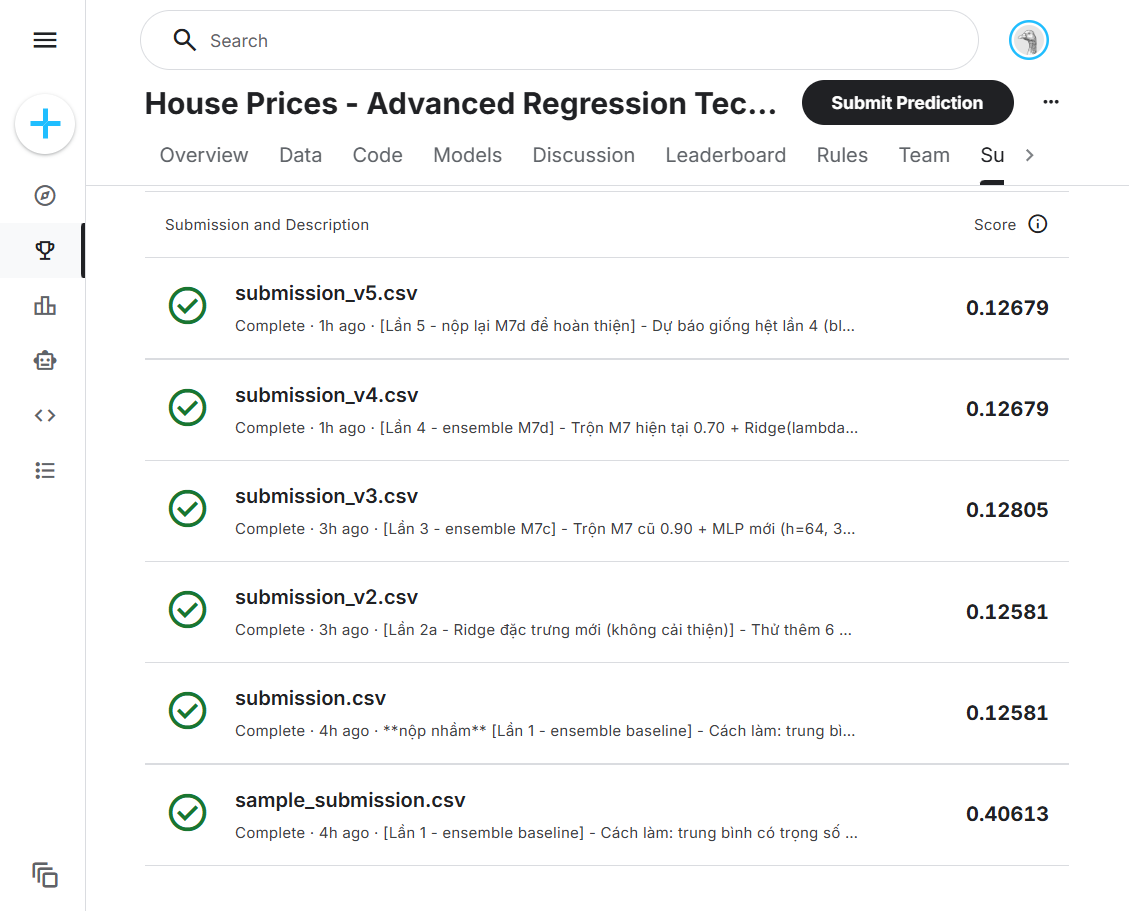
\includegraphics[width=0.95\textwidth]{kaggle_submissions.png} \\
{\small Minh chứng nộp bài: 6 lần nộp trên Kaggle (lần đầu nhầm file mẫu).}
\end{center}

\newpage
\section{Vòng lặp cải tiến}

Sau lần nộp đầu (LB 0.12581), nhóm lặp đúng 1 cải tiến mỗi vòng, dừng khi 2 vòng liên tiếp
không tiến bộ:

\begin{itemize}
  \item \textbf{Vòng 2 — thêm 6 đặc trưng (TotalSF, tuổi nhà, QualArea...) + Ridge: thất bại.}
        Ridge mới (0.11201) thua Ridge cũ (0.11193): TotalSF chỉ là cộng 2 cột cũ lại
        (tuyến tính tự cộng được), QualArea là phép nhân mà đường thẳng không hiểu.
        Trộn ra 100\% cũ + 0\% mới nên \textbf{không nộp}.
  \item \textbf{Vòng 3 — MLP + đặc trưng mới: thắng.} M4b đạt 0.12397 (hơn M4 cũ 0.12520):
        mạng nơ-ron ăn được phép nhân QualArea. Trộn M7c (0.11128) và nộp lần 3,
        nhưng LB 0.12805 không theo — cải thiện OOF quá nhỏ, chỉ là nhiễu.
  \item \textbf{Vòng 4 — Ridge phạt mạnh ($\lambda=30$): thắng nửa vời.} Một mình chỉ
        0.11222 nhưng sai khác hướng với M7 nên trộn M7d đạt 0.11103 — bài học:
        thành viên ensemble không cần giỏi hơn, chỉ cần sai khác nhau. LB lần 4: 0.12679.
  \item \textbf{Vòng 5 — seed-ensemble M4: nửa thắng nửa thua.} Trung bình 3 seed đạt
        0.12291 (hơn M4 đơn) nhưng trộn vào M7d vẫn 100\% cũ + 0\% mới.
        \textbf{Dừng vòng lặp}, nộp lại M7d làm lần 5 cho hoàn thiện (LB 0.12679).
\end{itemize}

Bài học lớn nhất: đặc trưng mới chỉ phát huy khi gặp đúng mô hình, và săn từng 0.000x
trên CV rất dễ tự lừa mình — phải để LB thật phán xử.

\newpage
\section{Kết luận}

Nhóm đã hoàn thành bài toán dự báo giá nhà theo đúng 6 bước CRISP-DM, toàn bộ mô hình bằng
PyTorch: EDA phát hiện giá lệch phải và đa cộng tuyến; pipeline 6 bước cho ra ma trận
$1456 \times 302$; fine-tune 2 vòng trên 8 họ mô hình (70 thí nghiệm có nhật ký);
ensemble M7 (Ridge 0.9 + M6 0.1) đạt CV 0.11140 và \textbf{LB public 0.12581} sau 5 lần nộp.

Hạn chế: chênh CV--LB khoảng 0.014 (overfit nhẹ); dữ liệu chỉ 1456 dòng nên mạng sâu và
embeddings chưa phát huy hết; 4/6 đặc trưng mới không thêm thông tin cho mô hình tuyến tính.
Hướng tiếp theo: stacking có meta-learner, mã hóa thứ tự cho biến ordinal, và thử
gradient boosting làm thành viên ensemble ngoài PyTorch để đối chứng.

\end{document}
